\documentclass[a4paper,twocolumn]{article}
\usepackage{enumitem}
\usepackage{tikz}
\usetikzlibrary{arrows,automata}
\usepackage{graphicx}
\usepackage{mathtools}
\usepackage{marvosym}
\usepackage[utf8]{inputenc}
\usepackage[T1]{fontenc}
\usepackage[a4paper, top=0.8in, bottom=1.0in, left=0.8in, right=0.8in]{geometry}
\usepackage{amssymb}
\usepackage{amsmath}
\usepackage{amsthm}
\usepackage{verbatim}
\usepackage{minted}

\setcounter{secnumdepth}{0}


\begin{document}

\title{A Introduction to an Algebra of labelled Graphs}
\author{Anton Lorenzen}
\date{March 2018}

\maketitle

The algebraic-graphs package, or just alga, is a library for constructing graphs in Haskell using a functional interface.
This is a ground up introduction to alga. You should definitely read it from the beginning on though, even if
you have already read the original functional pearl\footnote{https://github.com/snowleopard/alga-paper} since some definitions are different. 

\section{A Introduction to Algebraic Graphs}

Think of any (finite) graph. As you probably know a graph can be represented as a matrix.
Let's say we have the vertices $V = (a, b, c, d, e)$:

\begin{center}
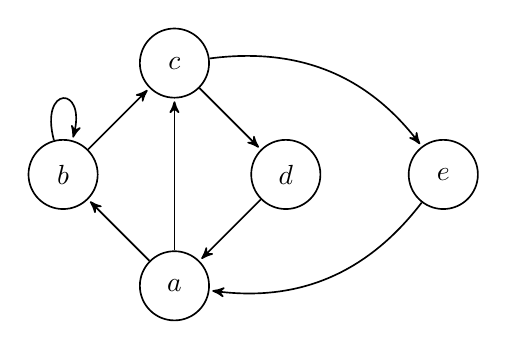
\begin{tikzpicture}[->,>=stealth',shorten >=1pt,auto,node distance=2.0cm,
                    semithick]

  \node[state] (C)                    {$c$};
  \node[state] (B) [below left  of=C] {$b$};
  \node[state] (D) [below right of=C] {$d$};
  \node[state] (A) [below right of=B] {$a$};
  \node[state] (E) [right of=D]       {$e$};

  \path (A) edge              node {} (B)
            edge              node {} (C)
        (B) edge [loop above] node {} (B)
            edge              node {} (C)
        (C) edge              node {} (D)
            edge [bend left]  node {} (E)
        (D) edge              node {} (A)
        (E) edge [bend left]  node {} (A);
\end{tikzpicture}
\end{center}

This is equivalent to the following matrix:

\[ A=
\begin{bmatrix}
  0 & 1 & 1 & 0 & 0 \\
  0 & 1 & 1 & 0 & 0 \\
  0 & 0 & 0 & 1 & 1 \\
  1 & 0 & 0 & 0 & 0 \\
  1 & 0 & 0 & 0 & 0
\end{bmatrix}
\]

We can decompose $A$ into 25 matrices each containing one of $A$'s elements and zeros everywhere else:

\[ A=
\begin{bmatrix}
  0 & 0 & 0 & 0 & 0 \\
  0 & 0 & 0 & 0 & 0 \\
  0 & 0 & 0 & 0 & 0 \\
  0 & 0 & 0 & 0 & 0 \\
  0 & 0 & 0 & 0 & 0
\end{bmatrix}
+ 
\begin{bmatrix}
  0 & 1 & 0 & 0 & 0 \\
  0 & 0 & 0 & 0 & 0 \\
  0 & 0 & 0 & 0 & 0 \\
  0 & 0 & 0 & 0 & 0 \\
  0 & 0 & 0 & 0 & 0
\end{bmatrix}
+ \dots
\]

TODO: (also note that $A + A = A$, since $1$ is the maximum element in each cell).

We can write each of these matrices as $FromVertex\xrightarrow{}ToVertex$
in the case of a $1$ and $\varepsilon$ in the case of a zero.
Therefore we have:

\[ A = \varepsilon + a\xrightarrow{}b + \dots \]

We can therefore represent every matrix using the following data type:
\begin{minted}{haskell}
newtype Vertex a = Vertex a

data Graph a = Empty
  | Connect Vertex Vertex
  | Overlay (Graph a) (Graph a)
\end{minted}

Here \texttt{Connect} corresponds to $\xrightarrow{}$, \texttt{Empty} to $\varepsilon$ and \texttt{Overlay} to $+$.
We require that \texttt{Overlay} is associative, commutative, has \texttt{Empty} as an identity element
and is idempotent ($a\xrightarrow{}b + a\xrightarrow{}b = a\xrightarrow{}b$) just like our matrix addition above.

Now, this isn't too revolutionary since we are basically just building an unbalanced binary tree of edges.
But it gets more interesting if we allow \texttt{Connect} to connect more than simple vertices.
For example, maybe we could define the following:
\begin{minted}[escapeinside=~~]{haskell}
data Graph a = ~$\varepsilon$~
  | Vertex a
  | (Graph a) ~$\xrightarrow{}$~ (Graph a)
  | (Graph a) ~$+$~ (Graph a)

[x,y,z] = map Vertex ["x", "y", "z"]
\end{minted}
With the law:
\begin{minted}[escapeinside=~~]{haskell}
x ~$\xrightarrow{}$~ (y ~$+$~ z) == (x ~$\xrightarrow{}$~ y) ~$+$~ (x ~$\xrightarrow{}$~ z)
(x ~$+$~ y) ~$\xrightarrow{}$~ z == (x ~$\xrightarrow{}$~ z) ~$+$~ (y ~$\xrightarrow{}$~ z)
\end{minted}
That opens up the question what
\begin{minted}[escapeinside=~~]{haskell}
x ~$\xrightarrow{}$~ y == x ~$\xrightarrow{}$~ (y ~$+$~ ~$\varepsilon$~)
       == (x ~$\xrightarrow{}$~ y) ~$+$~ (x ~$\xrightarrow{}$~ ~$\varepsilon$~)
\end{minted}
means for the $x \xrightarrow{} \varepsilon$ part?
Obviously, it needs to be $\varepsilon$, you might say and you would end up with
a $\xrightarrow{}$ that looks pretty much like matrix multiplication.
But alga took a different route and added another law, which gives it a different spin:
\begin{minted}[escapeinside=~~]{haskell}
x ~$\xrightarrow{}$~ ~$\varepsilon$~ == ~$\varepsilon$~ ~$\xrightarrow{}$~ x == x
x ~$\xrightarrow{}$~ (y ~$\xrightarrow{}$~ z) == (x ~$\xrightarrow{}$~ (y ~$+$~ z)) ~$+$~ (y ~$\xrightarrow{}$~ z)
(x ~$\xrightarrow{}$~ y) ~$\xrightarrow{}$~ z == ((x ~$+$~ y) ~$\xrightarrow{}$~ z) ~$+$~ (x ~$\xrightarrow{}$~ y)
\end{minted}
This law is what makes alga different from existing approaches, because it does it away with the difference between vertices and edges:
The $\xrightarrow{}$ constructor of the graph preserves the vertices contained in it. We can even derive this property from the laws:

\begin{align*}
  x \xrightarrow{} y &= (x \xrightarrow{} y) \xrightarrow{} \varepsilon \\
  &= ((x + y) \xrightarrow{} \varepsilon) + (x \xrightarrow{} y) \\
  &= x + y + (x \xrightarrow{} y)
\end{align*}

Convince yourself that we can see $x$ and $y$ as arbitrary graphs from now on and not just as vertices.
Also we will assume that $\xrightarrow{}$ binds stronger than $+$.

So, what is a good intuition for $\xrightarrow{}$? To come back to your $A$ matrix above, we can write

\[ (a + b) \xrightarrow{} (d + e) = 
\begin{bmatrix}
  0 & 0 & 0 & 1 & 1 \\
  0 & 0 & 0 & 1 & 1 \\
  0 & 0 & 0 & 0 & 0 \\
  0 & 0 & 0 & 0 & 0 \\
  0 & 0 & 0 & 0 & 0
\end{bmatrix}
\]

Exercises:
\begin{itemize}
\item Show that the laws imply that $\xrightarrow{}$ is associative.
\item Show that the idempotence of $+$ and $\varepsilon$ being the identity of $+$ follow from the other laws.
\item Show that $x \xrightarrow{} x \xrightarrow{} x = x \xrightarrow{} x$.
\item Show we can derive the decomposition law from the original paper:
  \[ a \xrightarrow{} b \xrightarrow{} c = a \rightarrow{} b + a \xrightarrow{} c + b \xrightarrow{} c \]
\end{itemize}

\subsection{About intuition}

Now that you have worked through the exercises, you will probably agree
that we can characterize a graph by the following laws:
\begin{itemize}
\item Addition: $+$ is associative and commutative.
\item Identity: $\varepsilon$ is the identity of $\xrightarrow{}$.
\item Distribution:
  \begin{align*} 
    x \xrightarrow{} (y + z) &= (x \xrightarrow{} y) + (x \xrightarrow{} z) \\
    (x + y) \xrightarrow{} z &= (x \xrightarrow{} z) + (y \xrightarrow{} z)
  \end{align*}
\item Extraction:
  \begin{align*}
    x \xrightarrow{} (y \xrightarrow{} z) &= (x \xrightarrow{} (y + z)) + (y \xrightarrow{} z) \\
    (x \xrightarrow{} y) \xrightarrow{} z &= ((x + y) \xrightarrow{} z) + (x \xrightarrow{} y)
  \end{align*}
\end{itemize}

The intuition I gave for these laws above might help you to understand what these laws mean in the contexts of graphs
and indeed all implementations of these laws as adjacency maps or sets follow this intuition.
However it falls short, if we go outside the context of graphs, so I would like to show you some statements you can't derive from the laws:
\begin{itemize}
\item \textit{$+$ and $\xrightarrow{}$ are distinct}. More specifically,
  every associative, commutative, idempotent operation with an identity fulfills the laws.
\item \textit{$\varepsilon$ denotes the empty matrix}. Consider for example $a + b = a \xrightarrow{} b = \text{min}(a,b)$
  with the identity being $\infty$.
\end{itemize}

\section{Labelled Graphs}

Let's go back to our graph from the beginning and add labels to the edges.

\begin{center}
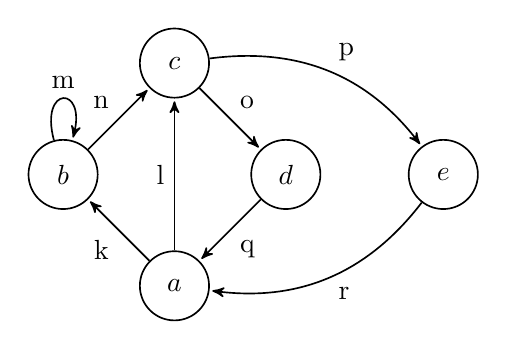
\begin{tikzpicture}[->,>=stealth',shorten >=1pt,auto,node distance=2.0cm,
                    semithick]

  \node[state] (C)                    {$c$};
  \node[state] (B) [below left  of=C] {$b$};
  \node[state] (D) [below right of=C] {$d$};
  \node[state] (A) [below right of=B] {$a$};
  \node[state] (E) [right of=D]       {$e$};

  \path (A) edge              node {k} (B)
            edge              node {l} (C)
        (B) edge [loop above] node {m} (B)
            edge              node {n} (C)
        (C) edge              node {o} (D)
            edge [bend left]  node {p} (E)
        (D) edge              node {q} (A)
        (E) edge [bend left]  node {r} (A);
\end{tikzpicture}
\end{center}

This is equivalent to the following matrix:

\[ A=
\begin{bmatrix}
  0 & k & l & 0 & 0 \\
  0 & m & n & 0 & 0 \\
  0 & 0 & 0 & o & p \\
  q & 0 & 0 & 0 & 0 \\
  r & 0 & 0 & 0 & 0
\end{bmatrix}
\]

Here you can think of $k, l, m, \dots$ as variable names standing for strings, numbers or anything else.
We will come back to which elements exactly we can use here in a minute.

Again we can decompose $A$ into 25 matrices each containing one of $A$'s elements and zeros everywhere else:

\[ A=
\begin{bmatrix}
  0 & 0 & 0 & 0 & 0 \\
  0 & 0 & 0 & 0 & 0 \\
  0 & 0 & 0 & 0 & 0 \\
  0 & 0 & 0 & 0 & 0 \\
  0 & 0 & 0 & 0 & 0
\end{bmatrix}
+ 
\begin{bmatrix}
  0 & k & 0 & 0 & 0 \\
  0 & 0 & 0 & 0 & 0 \\
  0 & 0 & 0 & 0 & 0 \\
  0 & 0 & 0 & 0 & 0 \\
  0 & 0 & 0 & 0 & 0
\end{bmatrix}
+ \dots
\]

And write each of these matrices as $FromVertex\xrightarrow{edge}ToVertex$.
Therefore we have:

\[ A = a\xrightarrow{0}a + a\xrightarrow{k}b + \dots \]

We can therefore represent every labelled graph as the following data type:
\begin{minted}[escapeinside=~~]{haskell}
data Graph l a = ~$\varepsilon$~
  | Vertex a
  | (Graph a) ~$\xrightarrow{l}$~ (Graph a)
  | (Graph a) ~$+$~ (Graph a)

[x,y,z] = map Vertex ["x", "y", "z"]
[k,l,m,n] = ["k", "l", "m", "n"]
\end{minted}

With the new laws:
\begin{itemize}
\item Addition: $+$ is associative and commutative.
\item Identity: $\varepsilon$ is the identity of $\xrightarrow{l}$.
\item Distribution:
  \begin{align*} 
    x \xrightarrow{k} (y + z) &= (x \xrightarrow{k} y) + (x \xrightarrow{k} z) \\
    (x + y) \xrightarrow{k} z &= (x \xrightarrow{k} z) + (y \xrightarrow{k} z)
  \end{align*}
\item Extraction:
  \begin{align*}
    x \xrightarrow{k} (y \xrightarrow{l} z) &= (x \xrightarrow{k} (y + z)) + (y \xrightarrow{l} z) \\
    (x \xrightarrow{k} y) \xrightarrow{l} z &= ((x + y) \xrightarrow{k} z) + (x \xrightarrow{l} y)
  \end{align*}
\item Absorption:
  \begin{align*}
    x \xrightarrow{k} y + x \xrightarrow{l} y &= x \xrightarrow{k + l} y
  \end{align*}
\end{itemize}

Exercise: Under which circumstances is the new $\xrightarrow{l}$ still associative?

\subsection{Semirings}

You have probably noticed that we used a new $+$ operation on our labels above
and as you might have guessed there are laws for it too, since we might run into contradictions otherwise:
\begin{itemize}
\item $+$ is commutative, associative and idempotent.
\item There is an element called $0$ which acts as an identity for $+$.
\end{itemize}

\end{document}
